\documentclass[tikz]{standalone}

\usepackage{tikz}
\usetikzlibrary{automata}

\begin{document}

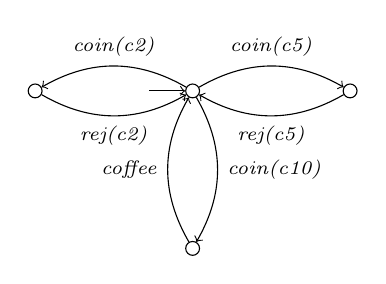
\begin{tikzpicture}
    \tikzstyle{every state}=[
        draw,
        shape=circle,
        inner sep=1pt,
        minimum size=5pt,
        final/.style={double,minimum size=6pt},
        initial text=]
        
    [auto,->]
    \renewcommand{\a}[1]{\textit{#1}}
    \node[state,initial] (n0) at (0,0) {};
    \node[state] (n2) at (-2,0) {};
    \node[state] (n10) at (0,-2) {};
    \node[state] (n5) at (2,0) {};

    \path[->]
    (n0) edge[bend right] node[above] {\scriptsize{\a{coin(c2)}}} (n2)
    (n2) edge[bend right] node[below] {\scriptsize{\a{rej(c2)}}} (n0)
    (n0) edge[bend left] node[above] {\scriptsize{\a{coin(c5)}}} (n5)
    (n5) edge[bend left] node[below] {\scriptsize{\a{rej(c5)}}} (n0)
    (n0) edge[bend left] node[right] {\scriptsize{\a{coin(c10)}}} (n10)
    (n10) edge[bend left] node[left] {\scriptsize{\a{coffee}}} (n0);
\end{tikzpicture}
\end{document}